% Name your report <group>-<unique-name>.tex, (e.g., sls-jupiter.tex)
% to avoid name collisions.  For \label{} entries within a file,
% please use \<group>-<unique-name>-<your label} (e.g.,
% \label{sls-jupiter-figure}), again to avoid name collisions.  There
% is no need to use unique names with \cite{} since each report has
% its own citation namespace.

% Normally, you would use \formattitlecontents{Title}{Authors},
% but in this case we needed footnotes in the author list to indicate
% visiting scientists.  You might also want to use \formattitle if you
% wish to control line breaks in the title or author list.  Please do
% not put any special formatting in \formattitlecontents or
% \formatcontents as this will disturb the table of contents.

\formattitle%
  {StreamIt: A Language and Compiler for Streaming Applications}
  {Michael Gordon, Michal Karczmarek, David Maze, William Thies, and
  Saman Amarasinghe}

\formatcontents%
  {StreamIt: A Language and Compiler for Streaming Applications}
  {Michael Gordon, Michal Karczmarek, David Maze, William Thies, and
  Saman Amarasinghe}

% Please use the following \formatsection entries unless they are
% inappropriate: Introduction, Approach, Progress, Future, Research
% Support.
%
% Do not put a blank line after a \formatsection, as this affects the
% formatting.

\formatsection{Introduction}
Recent years have seen the proliferation of applications that are
based on some notion of a ``stream''.  There is evidence that
streaming media applications are already consuming most of the cycles
on consumer machines, and their use is continuing to grow.  The stream
abstraction is central to embedded applications for hand-held
computers, cell phones, and DSP's, as well as for high-performance
applications such as intelligent software routers, cell phone base
stations, and HDTV editing consoles.

The goal of the StreamIt project is to provide natural language
constructs and high-performance compiler technology for modern stream
programming.  Today, most programmers turn to general-purpose
languages such as C or C++ to implement stream programs, resorting to
low-level assembly codes for loops that require high performance.
This practice is labor intensive, error-prone, and very costly, since
the performance-critical sections must be re-implemented for each
target architecture.  The StreamIt language aims to provide natural,
high-level stream constructs that raise the abstraction level in the
streaming domain.  At the same time, the StreamIt compiler will
perform aggressive optimizations so that the abstractions do not
sacrifice performance.
%these high-level abstractions
%can be used without sacrificing performance.

In addition, StreamIt is designed to be portable across machines that
are most well-suited for stream processing, including the emerging
class of communication-exposed architectures such as Raw \cite{rawshort}.
Part of the success of the C language was that it provided a portable
interface for von-Neumann machines: it abstracted away the
idiosyncratic differences between one machine and another, but exposed
the common properties that were important for achieving good
performance.  In the same way, StreamIt aims to provide a portable
language for next-generation processors that have replicated
processing units with compiler-orchestrated communication.  The
StreamIt language abstracts away the granularity of a parallel
machine, but exposes the regular communication patterns and abundant
parallelism that are key to obtaining high performance.

\formatsection{Approach}
The StreamIt language is designed to satisfy two criteria: first, it
ought to provide high-level abstractions that improve programmer
productivity, and second, it should be amenable to straightforward
compiler analyses for achieving high performance.  While these goals
are often conflicting in the design of programming languages, the
salient features of StreamIt are beneficial to both ends.  These
features include the notion of an autonomous ``filter'' as the basic
stream component, a structured model of filter composition, a
messaging system for control, and a hierarchical re-initialization
mechanism.  The initial version of StreamIt consists of legal Java
syntax to minimize the entry barrier for experienced programmers.
However, in the future, we plan to design a more compact syntax that
is specifically designed for streaming programs.

The basic unit of computation in StreamIt is the {\tt Filter}, such as
the {\tt FIRFilter} illustrated in
Figure~\ref{fig:commit-streamit-firstreamit}.  Each {\tt Filter}
contains an {\tt init} function that is called at initialization time;
in this case, the {\tt FIRFilter} records the coefficients that it
should use for filtering.  The {\tt work} function describes the most
fine grained execution step of the filter in the steady state.  Within
the {\tt work} function, the filter can communicate with neighboring
blocks using the {\tt input} and {\tt output} channels, which are FIFO
queues with types as declared in the {\tt init} function.  These
high-volume channels support the intuitive operations of {\tt
push(value)}, {\tt pop()}, and {\tt peek(index)}, where {\tt peek}
returns the value at position $index$ without dequeuing an item.

In order to express a streaming computation, a set of filters must be
assembled into a stream graph.  Rather than allowing the user to
construct an arbitrary network of filters, StreamIt provides three
pre-defined stream structures that can be to construct hierarchical
stream graphs (see Figure~\ref{fig:commit-streamit-structures}).  The
comparison of StreamIt's structure with arbitrary stream graphs could
be likened to the difference between structured control flow and GOTO
statements.  Though sometimes the structure restricts the
expressiveness of the programmer, the gains in robustness,
readability, and compiler analysis are immense.

The most simple construct for filter composition is the {\tt
Pipeline}, such as the {\tt Main} class in Figure
\ref{fig:commit-streamit-firstreamit}.  Like a {\tt Filter}, a {\tt
Pipeline} has an {\tt init} function that is called upon its
instantiation.  However, there is no {\tt work} function, and all
input and output channels are implicit; the stream behaves as the
sequential composition of filters that are specified with successive
calls to {\tt add} from within {\tt init}.  In addition to the {\tt
Pipeline}, the {\tt SplitJoin} construct can be used to specify
independent parallel streams that diverge from a common {\it splitter}
and merge into a common {\it joiner}, while the {\tt FeedbackLoop}
construct provides a way of introducing cycles in the stream graph.

While the {\tt input} and {\tt output} channels provide a way for
filters to communicate with their neighbors in the steady state,
StreamIt also provides a dynamic messaging system for passing
irregular, low-volume control information between non-neighboring
filters.  
%Messages are sent from within the body of a filter's {\tt
%work} function, perhaps to change a parameter in another filter.  
The most important difference between a message and a traditional
function call is that a message is asynchronous--there is no return
value associated with a message, and the callee can continue to
execute while the message is en route.  This is important in a
distributed environment, since a synchronous interaction between
processors imposes a high synchronization overhead.

%However, StreamIt
%does allow the caller to control the timing of message delivery via a
%sophisticated mechanism that is based on the flow of data items
%through the stream.  For instance, an upstream filter $A$ can signal a
%downstream filter $B$ to change its network protocol when it first
%sees the ``effects'' of the current data item that $A$ is processing.

\begin{figure}[t]
\centering
\begin{minipage}{2.5in}
  \includegraphics[width=61.42mm]{cag-commit-streamit-fir.eps}
%\psfig{figure=fir-streamit.eps,width=61.42mm}
\\
\caption{\protect\small An FIR filter in StreamIt.~~~~~
\protect\label{fig:commit-streamit-firstreamit}}
\end{minipage}
\begin{minipage}{3in}
\centering
\vspace{10pt}
  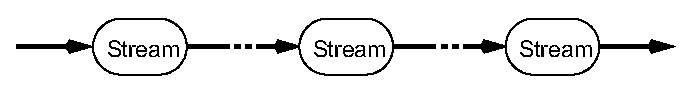
\includegraphics[width=1.8in]{cag-commit-streamit-pipeline.eps}
%\psfig{figure=basic-pipeline.eps,width=1.8in}

(a) A Pipeline. \\
\vspace{10pt}
  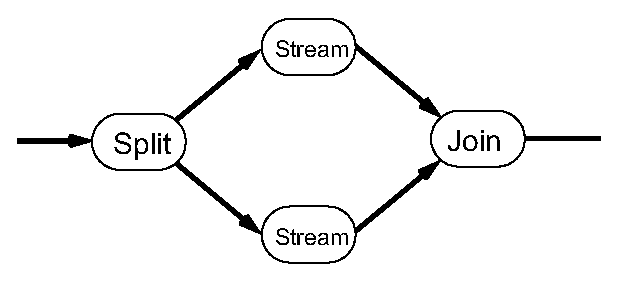
\includegraphics[width=1.8in]{cag-commit-streamit-splitjoin.eps}
%\psfig{figure=basic-splitjoin.eps,width=1.8in}

(b) A SplitJoin. \\
\vspace{10pt}
  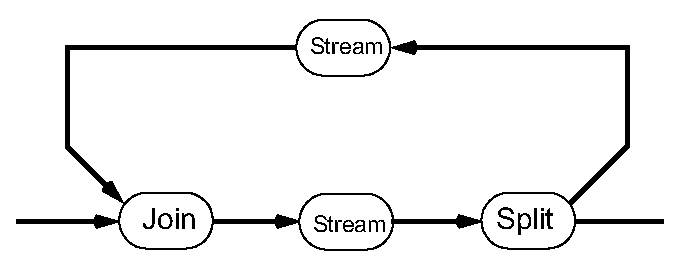
\includegraphics[width=1.8in]{cag-commit-streamit-feedback.eps}
%\psfig{figure=basic-feedback.eps,width=1.8in}

(c) A FeedbackLoop. \\
\caption{\protect\small Stream structures supported by StreamIt.
\protect\label{fig:commit-streamit-structures}
}
\end{minipage}
\vspace{-6pt}
\end{figure}

\formatsection{Progress} We have implemented a fully-functional
prototype of the StreamIt optimizing compiler as an extension to the
KOPI compiler infrastructure.  We can generate code for a uniprocessor
which performs comparably to SpectrumWare \cite{spectrumware}, a
streaming runtime library implemented in C++.

We are currently implementing a backend for the Raw processor
\cite{rawshort}, which supports fine-grained compiler-controlled
communication between tiled processing units.  A focus of our current
work is on developing fission and fusion algorithms that adjust the
granularity of the stream graph to match that of a given target.  For
example, if the granularity of the target exceeds that of the program,
then stateless filters can be duplicated across a {\tt SplitJoin} that
runs on multiple processors, and large filters can be split up into a
{\tt Pipeline} that spans several processing units.  Conversely, if
the granularity of the program exceeds that of the target, then
filters can be fused into a single stream construct that can execute
on a given processor.

\formatsection{Future} The primary focus of future work is
optimization.  Many streaming applications require high performance,
and they execute on embedded environments with limited resources.
Thus, there are many metrics by which to optimize, including
throughput, latency, code size, and data size.  Moreover, there are
great opportunities for novel stream-specific optimizations in
StreamIt, as the structured stream graph exposes the regular
communication patterns and widespread parallelism that are intrinsic
to stream programs but are often obscured in general-purpose
programming languages such as C or C++.

In addition, the current version of StreamIt requires that the I/O
rates of each filter must be known at compile-time.  In the future, we
plan to extend StreamIt to support dynamically varying data rates.

\formatsection{Research Support}
This research is supported in part by the MIT Oxygen Project, and by
DARPA under contract DBT6396-C-0036.

% Although the use of BibTeX is highly recommended, you can manually
% format your references as follows:
%
% \begin{thebibliography}{1}
%
% \bibitem{Zue00}
% V.~Zue, S.~Seneff, J.~R. Glass, J.~Polifroni, C.~Pao, T.~J. Hazen, and
% L.~Hetherington, ``\textsc{Jupiter}: A telephone-based conversational
% interface for weather information,'' \textit{IEEE Transactions on
% Speech and Audio Processing}, vol. 8, no.  1, pp. 85--96, Jan. 2000.
% 
% \end{thebibliography}

\bibtex{cag-commit-streamit}
